\documentclass[10pt,a4paper]{book}

\usepackage[utf8]{inputenc}
\usepackage[english]{babel}
\usepackage[english]{isodate}
\usepackage[parfill]{parskip}
\usepackage{tikz}
\usetikzlibrary{decorations.pathreplacing,shapes,arrows,positioning}
\usetikzlibrary{positioning}

\tikzstyle{input} = [coordinate]
\tikzstyle{output} = [coordinate]
\tikzstyle{block} = [rectangle, draw, text width=5em, text centered,  minimum height=4em]
\tikzstyle{storage} = [cylinder, shape border rotate=90, aspect=0.25, draw]
\begin{document}
% \maketitle\tableofcontents\newpage
\pagenumbering{Roman}
\tableofcontents
\newpage
% \listoffigures
% \newpage
% \listoftables
% \newpage
\pagenumbering{arabic}

\chapter{Planing}
\section{Idea}
\section{System diagram}
\begin{figure}[h!]
% \centered
\small
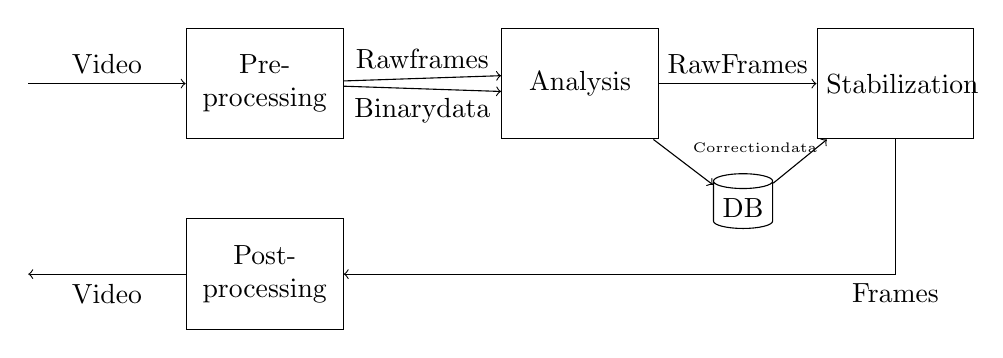
\begin{tikzpicture}[node distance=1cm and 2cm,auto]
    \node [input, name=input] {};
    \node [block, right= of input] (pre) {Pre-processing};
    \node [block, right= of pre] (analysis) {Analysis};
    \node [block, right= of analysis] (stabi) {Stabilization};
    \node [block, below= of pre] (post) {Post-processing};
    \node [input, left=of post] (output) {t};

    \node [storage, below right=0.5cm and 0.7cm of analysis] (analysisstorage) {DB};

     \draw[->](input) -- node {Video}(pre);
     \draw[->]([yshift=0.4cm]pre) -- node {Rawframes}(analysis);
     \draw[->]([yshift=-0.4cm]pre) -- node[below]{Binarydata}(analysis);
     \draw[->](analysis) -- node {RawFrames}(stabi);
     \draw[->](analysis) -- node {\tiny Correctiondata}(analysisstorage);
     \draw[->](analysisstorage) -- node {}(stabi);
     \draw[->](stabi) |- node {Frames}(post);
     \draw[->](post) -- node {Video}(output);
\end{tikzpicture}
\caption{High-level system diagram}
\end{figure}

%%%%%%%%%%%%%%%%%%%%%%%%%%%%%%%%%%%%%%%%%%%%%%%%%%%%%%%%%%%%%%%%%%%%%%%%%%%%%%%%
%%%%%%%%%%%%%%%%%%%%%%%%%%%%%% LOWER LEVEL SD %%%%%%%%%%%%%%%%%%%%%%%%%%%%%%%%%%
%%%%%%%%%%%%%%%%%%%%%%%%%%%%%% Preprocessing  %%%%%%%%%%%%%%%%%%%%%%%%%%%%%%%%%%
%%%%%%%%%%%%%%%%%%%%%%%%%%%%%%%%%%%%%%%%%%%%%%%%%%%%%%%%%%%%%%%%%%%%%%%%%%%%%%%%

\begin{figure}[h!]
% \centered
\small
\begin{tikzpicture}[node distance=1cm and 2cm,framed,background rectangle/.style={dotted,thick,draw=gray,rounded corners},auto]
    \node [input, name=input] {};
    \node [block, right= of input] (extract) {Extraction of single frames \textit{\small \color{gray} Decoding}};
    \node [block, right= of extract] (color) {Color handling};
    \node [block, below= of color] (binary) {Binary conversion};
    \node [input, below= 2.275cm of input] (output) {t};

    % \node [storage, below right=0.5cm and 0.7cm of analysis] (analysisstorage) {DB};

     \draw[->](input) -- node {Video}(extract);
     \draw[->](extract) -- node {Rawframes}(color);
     \draw[->](color) -- node {Frames}(binary);

     \draw[->](extract) |- ++(0,1cm) -- ++(8cm,0) |- ++(0,-4.1cm) -- node[below]{Rawframes} ++(-11cm,0);

     \draw[->](binary) -- node {Binarydata}(output);
\end{tikzpicture}
\caption{Detailed system diagram of the \textit{Preprocessing}}
\end{figure}

%%%%%%%%%%%%%%%%%%%%%%%%%%%%%%%%%%%%%%%%%%%%%%%%%%%%%%%%%%%%%%%%%%%%%%%%%%%%%%%%
%%%%%%%%%%%%%%%%%%%%%%%%%%%%%%%%% Analysis %%%%%%%%%%%%%%%%%%%%%%%%%%%%%%%%%%%%%
%%%%%%%%%%%%%%%%%%%%%%%%%%%%%%%%%%%%%%%%%%%%%%%%%%%%%%%%%%%%%%%%%%%%%%%%%%%%%%%%

\begin{figure}[h!]
% \centered
\small
\begin{tikzpicture}[node distance=1cm and 2cm,framed,background rectangle/.style={dotted,thick,draw=gray,rounded corners},auto]
    \node [input, name=input] {};
    \node [block, right= of input] (local) {Local Motion Estimation};
    \node [block, below right= of input, color=gray, dotted] (global) {Global Motion Estimation};
    \node [block, right= of local] (motionsmootinglocal) {Motion smoothing};
    \node [block, right= of global, color=gray, dotted] (motionsmootingglobal) {Motion smoothing};
    \node [block, right= of motionsmootinglocal] (aggr) {Aggregation};
    \node [input, below left=of global] (output) {t};

    % \node [storage, below right=0.5cm and 0.7cm of analysis] (analysisstorage) {DB};

     % \draw[->](input) --  ++(0.5cm,-0.2cm) -| node[midway left]{Frames} ++(1cm,-1.9cm) --  (output);
     \draw[->](input) -- node{Binarydata}(local);
     \draw[->, color=gray](input) -- node[below left]{Binarydata}(global);
     \draw[->](local) -- node[above]{\scriptsize Correctiondata}(motionsmootinglocal);
     \draw[->, color=gray](global) -- node[below]{\scriptsize Correctiondata}(motionsmootingglobal);
     \draw[->](motionsmootinglocal) -- node[above]{\scriptsize Correctiondata}(aggr);
     \draw[->, color=gray](motionsmootingglobal) -- node[below right]{\scriptsize Correctiondata}(aggr);

     \draw[->](aggr) |- node[above left]{Correctiondata}(output);

     \draw[->](input) |-  ++(0,1cm) -- ++(12cm,0) |- ++(0,-4.5cm) -- node[below]{Rawframes} ++(-12cm,0);
\end{tikzpicture}
\caption{Detailed system diagram of the \textit{Analysis}}
\end{figure}

%%%%%%%%%%%%%%%%%%%%%%%%%%%%%%%%%%%%%%%%%%%%%%%%%%%%%%%%%%%%%%%%%%%%%%%%%%%%%%%%
%%%%%%%%%%%%%%%%%%%%%%%%%%%%%%% Stabilization %%%%%%%%%%%%%%%%%%%%%%%%%%%%%%%%%%
%%%%%%%%%%%%%%%%%%%%%%%%%%%%%%%%%%%%%%%%%%%%%%%%%%%%%%%%%%%%%%%%%%%%%%%%%%%%%%%%

\begin{figure}[h!]
% \centered
\small
\begin{tikzpicture}[node distance=1cm and 2cm,framed,background rectangle/.style={dotted,thick,draw=gray,rounded corners},auto]
    \node [input, name=input] {};
    \node [block, right= of input] (transform) {Transform Rawframes};
    \node [input, name=output, right= of transform] {};

    % \node [storage, below right=0.5cm and 0.7cm of analysis] (analysisstorage) {DB};
    \draw[->]([yshift=0.1cm]input) -- node {Rawframes}(transform);
    \draw[->]([yshift=-0.1cm]input) -- node[below]{\scriptsize Correctiondata}(transform);
    \draw[->](transform) -- node[]{Frames}(output);


     % \draw[->](input) --  ++(0.5cm,-0.2cm) -| node[midway left]{Frames} ++(1cm,-1.9cm) --  (output);
\end{tikzpicture}
\caption{Detailed system diagram of the \textit{Stabilization}}
\end{figure}

%%%%%%%%%%%%%%%%%%%%%%%%%%%%%%%%%%%%%%%%%%%%%%%%%%%%%%%%%%%%%%%%%%%%%%%%%%%%%%%%
%%%%%%%%%%%%%%%%%%%%%%%%%%%%%% Postprocessing %%%%%%%%%%%%%%%%%%%%%%%%%%%%%%%%%%
%%%%%%%%%%%%%%%%%%%%%%%%%%%%%%%%%%%%%%%%%%%%%%%%%%%%%%%%%%%%%%%%%%%%%%%%%%%%%%%%

\begin{figure}[h!]
% \centered
\small
\begin{tikzpicture}[node distance=1cm and 2cm,framed,background rectangle/.style={dotted,thick,draw=gray,rounded corners},auto]
    \node [input, name=input] {};
    \node [block, right= of input] (enc) {Encoding};
    \node [input, name=output, right= of enc] {};

    % \node [storage, below right=0.5cm and 0.7cm of analysis] (analysisstorage) {DB};
    \draw[->](input) -- node[]{Frames}(enc);
    \draw[->](enc) -- node[]{Video}(output);


     % \draw[->](input) --  ++(0.5cm,-0.2cm) -| node[midway left]{Frames} ++(1cm,-1.9cm) --  (output);
\end{tikzpicture}
\caption{Detailed system diagram of the \textit{Postprocessing}}
\end{figure}

%%%%%%%%%%%%%%%%%%%%%%%%%%%%%%%%%%%%%%%%%%%%%%%%%%%%%%%%%%%%%%%%%%%%%%%%%%%%%%%%
%%%%%%%%%%%%%%%%%%%%%%%%%%%%%% Resulting %%%%%%%%%%%%%%%%%%%%%%%%%%%%%%%%%%
%%%%%%%%%%%%%%%%%%%%%%%%%%%%%%%%%%%%%%%%%%%%%%%%%%%%%%%%%%%%%%%%%%%%%%%%%%%%%%%%
% \begin{tikzpicture}
%    \node (a) at (0,0)
%      {
%         \begin{tikzpicture}
%            \draw (0,0) circle (1cm);
%         \end{tikzpicture}
%      };
%     \node (b) at (a.south) [anchor=north,yshift=-1cm]
%      {
%         \tikz\fill[blue] (0,0) circle (0.7cm);
%      };
%    \draw [<->] (a)--(b);
% \end{tikzpicture}



\end{document}
